\documentclass[11pt]{article}

\usepackage[utf8]{inputenc}
\usepackage[francais]{babel}
\usepackage{graphicx}
\usepackage{wrapfig}
\usepackage{fullpage}

\usepackage[top=100pt,bottom=70pt,left=60pt,right=60pt]{geometry}

\usepackage{amsfonts,amssymb,amsmath,amsthm} 
\usepackage[colorlinks,urlcolor=blue,linkcolor=black,citecolor=gray]{hyperref}

\usepackage{tikz}


\newtheoremstyle{exostyle}
{\topsep}% espace avant
{}%{\topsep}% espace apres
{}% Police utilisee par le style de thm
{}% Indentation (vide = aucune, \parindent = indentation paragraphe)
{\bfseries}% Police du titre de thm
{.}% Signe de ponctuation apres le titre du thm
{ }% Espace apres le titre du thm (\newline = linebreak)
{\thmname{#1}\thmnumber{ #2}\thmnote{. \normalfont{\textit{#3}}}}% composants du titre du thm : \thmname = nom du thm, \thmnumber = numéro du thm, \thmnote = sous-titre du thm

\newtheoremstyle{exostyle*}
{\topsep}% espace avant
{}%{\topsep}% espace apres
{}% Police utilisee par le style de thm
{}% Indentation (vide = aucune, \parindent = indentation paragraphe)
{\bfseries}% Police du titre de thm
{.}% Signe de ponctuation apres le titre du thm
{ }% Espace apres le titre du thm (\newline = linebreak)
{\thmname{#1}\thmnote{. \normalfont{\textit{#3}}}}% composants du titre du thm : \thmname = nom du thm, \thmnumber = numéro du thm, \thmnote = sous-titre du thm


\newcommand{\R}{\ensuremath{\mathbb R}}
\newcommand{\PP}{\ensuremath{\mathbb P}}
\newcommand{\CC}{\ensuremath{\mathbb C}}
\newcommand{\N}{\ensuremath{\mathbb N}}
\newcommand{\ZZ}{\ensuremath{\mathbb Z}}
\newcommand{\ds}{\displaystyle}
\newcommand{\Mm}{\mathcal{M}}
\renewcommand{\Im}{{\mathrm{Im} \, }}
\newcommand{\bR}{\mathbb R}
\newcommand{\bN}{\mathbb N}

\theoremstyle{exostyle}
\newtheorem{exercice}{Exercice} 
\newtheorem{solution}{Solution}

\usepackage{titlesec}
\renewcommand{\thesection}{\Roman{section}}
\titleformat{\section}[display]
{\large\bfseries}
{\vspace{.5cm}\titlerule[1.pt]}
{-10pt}
{\filright \large \qquad \thesection\ \large\bfseries\filright}[{\vspace{1.5mm}\titlerule[1pt]\vspace{5mm}}]


\newcommand{\ZeroRoman}[1]{% 0 + \Roman
  \ifcase\value{#1}\relax 0\else% Chapter 0
  \Roman{#1}\fi}% All other chapters
\renewcommand{\thesection}{\ZeroRoman{section}}

\date{} 
\author{}


%#############################################################################################
\begin{document}
\selectlanguage{french}


\noindent 
Sorbonne Universit\'e - Université Paris Cité     \hfill   Ann\'ee 2022-2023 \\
Pr\'eparation \`a  l'agr\'egation        \hfill     Vendredi 14 avril 2023 \\ % \emph{Dur\'ee : 3h}
 %\hfill \emph{Calculatrices et t\'el\'ephones interdits} \\
\noindent {\rule{\textwidth}{.2mm}}\\[-5mm]
\begin{center}
{\large \textsc{Examen option B} }\\[-5mm]
\end{center}
\noindent {\rule{\textwidth}{.2mm}}\\[1cm]


{\bfseries Merci de r\'ediger les deux exercices sur deux copies s\'epar\'ees.}

\begin{exercice}

  Dans cet exercice, on s’intéresse au système différentiel suivant 
  \begin{equation}
    \label{eq:EDO}
    \left\lbrace
      \begin{aligned}
        u'(t) &= -u(t) - u^3(t) + 3u(t) v^2(t), \\
        v'(t) &= -v(t) + v^3(t) - 3v(t) u^2(t), 
      \end{aligned}\right.
  \end{equation}
  et $u(0) = u_0, v(0) = v_0$ avec $u_0\geq 0$ et $v_0 \geq 0$.
  \begin{enumerate}
  \item Montrer que le système différentiel~\eqref{eq:EDO} admet une unique solution maximale $(u,v)$.
  \item Montrer que si $u_0>0$ alors $u(t) > 0$ pour tout $t$ où $u$ est définie. 
  \item Déterminer les points d’équilibre $(u,v) \in \R_+^{2}$ \underline{($u,v \geq 0$)} du système différentiel~\eqref{eq:EDO}.
    \'Etudier leur stabilité.
  \item Calculer les isoclines et dessiner le portrait de phase dans le cadran $\R_+^2$.
  \item Montrer que si $(u_0,v_0) \in II$ où $II$ est la zone définie par 
    \[
      II = \Big\lbrace (u_0,v_0) \in [0,\infty[^2 \ \text{tel que} \ \frac{1}{3}(u^2_0+ 1) \leq  v_0^2 \leq 3u_0^2+1 \Big\rbrace  
    \]
    alors la solution maximale tend vers $(0,0)$ et qu’elle est définie sur $\mathbb{R}_+$. 

    \emph{Indication:} on pourra remarquer que $v$ décroissante sur son domaine de définition.

  \item \`A partir de maintenant et jusqu'\`a la fin, on suppose que $u_0 = 0$. On pose $\tilde{v} = v^2$. Montrer que $\tilde{v}$ est solution de $\tfrac{1}{2}\tilde{v}'(t) = -\tilde{v}+\tilde{v}^2$ et montrer que si $v_0<1$ (respectivement $v_0>1$) alors $\tilde{v}<1$ (respectivement $\tilde{v}>1$) sur son domaine de définition.
  \item {[\bf Bonus]} Résoudre l’équation différentielle v\'erifi\'ee par $\tilde{v}$. 
  \item {[\bf Bonus]} En déduire la solution maximale $v$ et montrer qu’il existe une solution qui tend vers l’infini en temps fini.
  \end{enumerate}
\end{exercice}


%%%%%%%%%%%%%%%%%%%%%%%%%%%%%%%%%%%%%%%%%%%%%%%%%%% 

\begin{exercice}
  Soient $m$ et $n$ deux entiers non nuls, $A\in \Mm_{m,n}(\bR)$, $b\in \bR^m$. On s'intéresse à déterminer le ou les minimiseur(s) de la fonction $f:\bR^n \rightarrow \bR$ définie par
$$f(x) = \frac{1}{2} \|A x-b\|_2^2 $$
où $\|\cdot \|_2$ est la norme euclidienne de $\bR^m$. \\
 On rappelle que $f$ est dite \emph{coercive} (ou \emph{infinie à l'infinie}) si 
  $$f(x) \to + \infty  \mbox{ lorsque }\|x\| \to +\infty.$$
  On rappelle aussi le résultat suivant (qui poura être utilisé sans le démontrer): pour  $A\in \Mm_{m,n}(\bR)$ et $A^t$ sa matrice transposée~:
  $$\ker(A)= \ker(A^t A) \qquad \mbox{et}\qquad \Im(A^t)= \Im(A^tA).$$
  
\medskip

{\bf I. Existence d'un minimiseur}
\begin{enumerate}
 \item Montrer que $f$ est  coercive si et seulement si $A$ est injective. 
       Que peut-on en déduire ?
%
 \item \label{q:calcul-gradient} 
 Après avoir justifié que $f$ est deux fois différentiable sur $\bR^n$, 
calculer la différentielle de $f$ en tout point  $x \in \bR^n$. En déduire que 
le gradient de $f$ et sa matrice hessienne en $x$ sont 
$$
\nabla f(x) = A^t A x - A^t b \qquad \mbox{et} \qquad H_{f}(x) =  A^t A.
$$
 %
 \item Déterminer si $f$ est convexe.
  %
  \item Donner une condition nécessaire pour que $x^* \in \bR^n$ soit un minimiseur local de $f$. Cette condition est-elle suffisante ? Le minimum est-il global ?
  %
  \item 
  Donner une condition suffisante sur $A$ pour que $f$ admette un unique minimiseur global. Dans ce cas, exprimer le minimiseur global.
  %Montrer que si $A$ est injective alors $f$ admet  un unique minimiseur global. Dans ce cas, exprimer le minimiseur global.
  %
  \item On suppose ici $A$ quelconque. Montrer qu'il existe au moins un minimiseur global à $f$, et caractériser un tel minimiseur.
\end{enumerate}  

{\bf II. Approximation du minimiseur} \\
On suppose dans cette partie que $f$ possède un unique minimiseur global noté $x^*$. Pour $x \in \bR^n$ donné,  on définit la fonction 
 $$ \varphi_x(t) = f(x-t\nabla f(x)).$$
%
\begin{enumerate}
\setcounter{enumi}{6}
%
 \item Soit $x\neq x^*$. Montrer qu'il existe $\varepsilon>0$ tel que pour tout $t\in ]0,\varepsilon[$,
 $$ f(x-t \nabla f(x)) <f(x).$$
 Comment interpréter cela ?
%
\item \'Etant donné $x_0\in \bR^n$, on introduit la suite $(x_n)_{n\in \bN}$ donnée par la méthode du gradient (à pas variable $t_n$) pour approcher $x^*$. \'Ecrire l'expression de la relation de récurrence donnant $x_{n+1}$ en fonction de $x_n$. 
%
\item On suppose dans cette question que $t_n=\tau >0$ ne dépend pas de $n$. 
\begin{enumerate}
   \item \'Ecrire explicitement la relation de récurrence donnant les itérés de la suite $(x_n)_{n\in \bN}$. 
    \item Montrer qu'en choissant $\tau$ suffisament petit   $x_n \to x^*$ lorsque $n\to +\infty$.
\end{enumerate}
 \item 
 \begin{enumerate}
   \item {[\bf Bonus]} Montrer que pour $x\neq x^*$,  $\varphi_x$ admet un unique minimiseur, noté $t^*_x$ sur $\bR$.
    \item {[\bf Bonus]} On  choisit maintenant $t_n =  t^*_{x_n}$. Quelle méthode numérique reconnaissez-vous ?
    \item {[\bf Bonus]} \`A l'aide d'un théorème du cours, justifiez la convergence de la suite $(x_n)_{n\in \bN}$ lorsqu'on prend  $t_n =  t^*_{x_n}$ (la preuve n'est pas demandée).
 \end{enumerate}   
\end{enumerate}
\end{exercice}




% #############################################################################################
\newpage

\noindent {\rule{\textwidth}{.2mm}}\\[-5mm]
\begin{center}
{\large \textsc{Corrigé examen option B} }\\[-5mm]
\end{center}
\noindent {\rule{\textwidth}{.2mm}}\\[1cm]

\begin{solution}
  \begin{enumerate}
  \item Application de Cauchy-Lipschitz local.
  \item Si $u(t)=0$ pour un certain temps $t$, alors $u=0$ est solution globale de l’EDO sur $u$.
  \item Les points d’équilibre tels que $u,v\geq 0$ sont $(0,0)$ et $(0,1)$ (la condition $-1-u^2+3v ^2=0$ et $-1+v^2-3u^2=0$ donne par différence $u^2+v^2=0$).
    Le Jacobien $JF(u,v) = \begin{bmatrix}
      -1-3u^2+3v^2 & 6uv \\
      6uv & -1-3v^2+3u^2
    \end{bmatrix}$, donc $JF(0,0) = \begin{bmatrix}
      -1 & 0 \\ 0 & -1
    \end{bmatrix}$ et $JF(0,1) = \begin{bmatrix}
      2 & 0 \\ 0 & 2
    \end{bmatrix}$. (0,0) est stable et (0,1) est instable.
  \item Les isoclines sont 
    \begin{itemize}
    \item $u (-1-u^2+3v^2) = 0 \Rightarrow$ $u=0$ ou $v = \frac{1}{\sqrt{3}} \sqrt{u^2+1}$
    \item $v (-1+v^2-3u^2) = 0 \Rightarrow$ $v=0$ ou $v =  \sqrt{3u^2+1}$
    \end{itemize}

    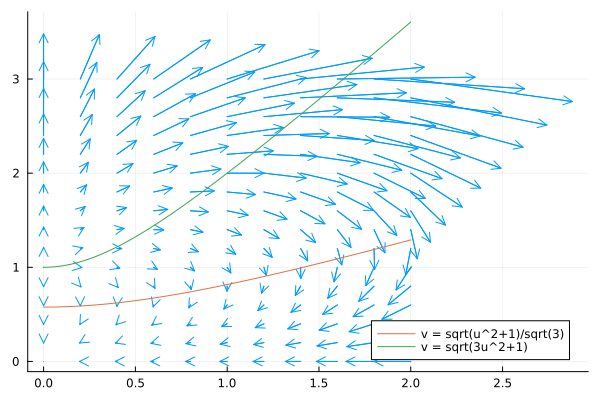
\includegraphics[width=0.5\textwidth]{portrait_phase.png}

  \item $v$ est décroissante et $(u,v)$ doit atteindre la zone $I = \Big\lbrace (u_0,v_0) \in [0,\infty[^2 \ \text{tel que} \ v_0^2 \leq \frac{1}{3}(u^2_0+ 1) \Big\rbrace$ (sinon il existerait un point d’équilibre avec $u>0$).
    Une fois dans $I$, $u$ est décroissante et le seul point d’équilibre dans la zone est $(0,0)$. La solution maximale est bornée donc définie sur $\mathbb{R}_+$

      \item $u = 0$ est solution globale de l’EDO sur $\R$, d’où l’EDO sur $\tilde{v}$. De même qu’avant $\tilde{v}=1$ est solution globale.

          \item 
    Par séparation de variables, on a (la constante $C$ n’est pas la même de ligne en ligne) si $v_0<1$
    \begin{align*}
      \frac{d\tilde{v}}{\tilde{v}^2-\tilde{v}} &= 2dt \\
      \frac{d\tilde{v}}{\tilde{v}} + \frac{d\tilde{v}}{1-\tilde{v}} & = -2dt \\
      \log(\tilde{v}) - \log(1-\tilde{v}) & = -2t + C \\
      \frac{\tilde{v}}{1-\tilde{v}} &=C \exp(-2t) \\
      -1+\frac{1}{\tilde{v}} &=C \exp(2t) \\
      \tilde{v} &= \frac{1}{1+C \exp(2t)}, C>0
    \end{align*}
    et la solution maximale est définie sur $\mathbb{R}$.
    
    Si $v_0>1$ alors 
    \begin{align*}
      \frac{d\tilde{v}}{\tilde{v}^2-\tilde{v}} &= 2dt \\
      \frac{d\tilde{v}}{\tilde{v}} + \frac{d\tilde{v}}{1-\tilde{v}} & = -2dt \\
      \log(\tilde{v}) - \log(\tilde{v}-1) & = -2t + C \\
      \frac{\tilde{v}}{\tilde{v}-1} &=C \exp(-2t) \\
      1-\frac{1}{\tilde{v}} &=C \exp(2t) \\
      \tilde{v} &= \frac{1}{1-C \exp(2t)},
    \end{align*}
    où $0<C<1$ pour satisfaire la condition initiale. $\tilde{v}$ explose en temps fini.
  \item Puisque $v>0$, on a $v = \sqrt{\tilde{v}}$ qui n’est définie que si $\tilde{v}$ est bien définie. Pour $v_0>1$, on a explosion en temps fini.
  \end{enumerate}
\end{solution}

\end{document}